
\section{Implementation}\label{sec:implementation}

In this chapter give some relevant implementation details, along with a diagram showing the pipeline of the system. \\

\subsection{From bills to news articles: modelling topics from bills }\label{subsec:topic}

In order to find entities that are related to the bills approved by a parliament, we need to find news articles that are related to the bills. To do this, we model a bill with a set of weighted keywords. These keywords can be used to query the corpus of news article and to rank the articles according to their relatedness to the bills. \\

To find keywords, we consider n-grams of size \emph{1,2,3}. We compute the TF-IDF score of these n-grams with respect to the set of all bills approved by the Parliament; that is, each bill constitutes one document. To enhance the quality of the keyword extraction we could also consider the transcripts of the debates of each bill; by doing this we could discover words and phrases that describe the contents of the bills in an informal, non-legislative way which is possibly more similar to the jargon used by newspapers. This is however a minor improvement and is left for future work. After extracting keywords, we rank them and keep the top 1024 keywords. We keep the TF-IDF score of the keywords as the weight of their association. \\

We used the extracted keywords to query the corpus of news articles. We index the news articles by extracting n-grams of size \emph{1,2,3} from the news articles and compute their TF-IDF score with respect to the whole set of news articles (one news article is one document). To find news articles related to the bills we compute the cosine similarity between the vectors representing the bills and the vectors representing the news articles. \\

To improve the phase of keyword extraction, we use Rocchio's algorithm to discover new keywords from the corpus of news articles. Rocchio's algorithm is widely used in Information Retrieval systems to expand queries defined by users by adding news terms found in the top relevant documents retrieved by an initial search. To determine what a relevant document is there are two alternatives: (i) asking the user for feedback - an option which is not possible in our application and ii) assume that the top documents retrieved by the query are relevant. \\

After defining a set of relevant documents $|R|$ and a set of non-relevant documents, we can update the query vector $q$ according to this formula: \\

\begin{eqnarray*}
q_{new} = \alpha* q +  \beta * \frac{1}{|R|} * \sum_{d \in R}{d} + \gamma * \frac{1}{|NR|} * \sum_{d \in NR}{d} \\
\end{eqnarray*}

Where d is a document in the Vector space model, $\alpha, \beta, \gamma $ are manually fixed parameters usually satisfying $\alpha > \beta > \gamma = 0$. \\

After a new query vector is computed, we execute a new query and rank the news articles according to the new query. After doing this, we need to determine the number of articles to use based on the score. There are many alternatives to address this problem; one way is to plot the score of the articles with respect to their ranking and find an elbow. The problem with this approach is that there is no clear definition of what an elbow is and consequently the methods chosen can perform better or worse according to the plot. To address this problem we choose the point at which the derivative is below a certain threshold, which is the point at which the curve ``flattens'' out. We provide an example with real data in figure \ref{fig:articles-topic-threshold}. \\

\begin{figure}[h!]
    \centering
    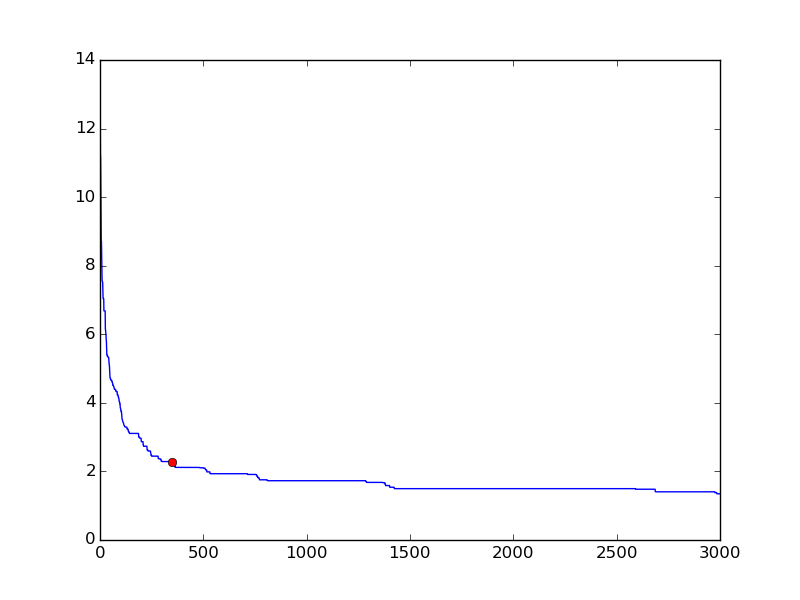
\includegraphics[width=0.7\textwidth]{figs/articles-topic-threshold}
    \caption{Determining the number of articles to use for a given bill.}
    \label{fig:articles-topic-threshold}
\end{figure}

\subsection{From news articles to political actors: entity recognition and preprocessing}\label{subsec:getting-entities}

After finding articles related to bills, they are analyzed to find entities that are in turn related to the bills. For this purpose we use MITIE, a state of art tool Named Entity Recognition tool created in the MIT. Given a document, MITIE identifies substrings that contain possible named entities and tags them as \emph{Organization, Location, Person} or \emph{Miscellaneous}.\\

Before carrying on the detected entities need to be pre-processed before they can be used. The names found may i) not be correctly delimited (resulting in truncated names or in names that contain excess text) ii) be ambiguous (an entity may have more than one name and a name may refer to more than one entity) and iii) may be noise and not refer to a real entity. \\

Name disambiguation is in itself a complex and interesting research topic which escapes the aim of this study. We have however implemented some heuristics we briefly describe below:\\

\begin{enumerate}

\item \textbf{Entity Normalization}: entities are brought to a canonical form to address spelling variations. This involves i) punctuation sign removal; ii) double, leading and trailing whitespaces removal; iii) leading and trailing stop words removal; iv) string camelization (all characters are put in lowercase except for the first letter of every word, which is in uppercase). 

\item \textbf{Mapping organization initials to the whole name}: when an organization name is detected we aim to detect if there are any other names composed by its initials. Specifically, we aim to exploit a widely found pattern: organizations often have the full name followed by the initials inside parenthesis. 

\item \textbf{Mapping partial names with full names}: when person names are detected we classify them into \emph{full names} (containing more than 1 word) and \emph{short names} (containing one word, which is possible the last or first name of the full name). We then link short names with the nearest, previous full name such that the short name is contained inside the full name.

\item \textbf{Expanding names based on the news corpus}: to address the issue of truncated names (eg 'Word Life Fund' may be truncated and processed as 'World and 'Life Fund')  we: i) look up every name and it's surrounding context in the corpus ii) extract sentences in the top articles and iii) find the longest substring matching these sentences. 
\end{enumerate}

By doing this we find a list of entities for which we have a list of aliases and a list of tags counts. After doing this, we choose for every entity the tag with the highest frequency as the type of the entity. \\

\subsection{Selecting relevant actors: scoring the relationship between an entity and a bill}\label{subsec:entity-bill-score}

After obtaining a list of entities for each bill, we need to measure the strength of the relationship between the entities and the topics. Our method for entity selection yields thousands of entities for each of the topics. This makes scoring the strength of the relationship necessary for two reasons.\\ 

First, noise is bound to be present in the list of entities found by our system. This includes entity names that do no correspond to real entities, entities that occur in articles related to the bills but that are not really related to them and entities from articles that are completely unrelated to the bills. By ranking the entities according to their relationship to the topics we can automatically or semi-automatically select the most relevant entities, thus performing noise reduction. \\

Second, to produce an entity-entity graph we need to compute similarity measures between each pair entities; the cost of each comparison depends on the method chosen and growths quadratically with the number of entities. This is particularly relevant if we want to use similarity measures based on a Web search engine. \\

To weight the relationship between an entity and a bill we have proposed a measure which takes into account three factors: the relationship between the article the entity occurs in and a bill; the frequency of an entity in that article and the frequency of an entity across the whole set of topics. Our measure follows the intuition of the TF-IDF weighting scheme: we want to give a high score to entities that occur frequently in articles highly related to bills and at the same time give lower scores to entities that occur in more than one topic. More formally we weight the relationship between an entity and a bill according to the following formula:


\begin{eqnarray*}
weight(e,t) = \sum_{\substack{n \in news(t), \\e \in n}}{\Big(\underbrace{log(cos\_similarity(n,t))}_{\text{news-topic similarity}}*\underbrace{log(freq(e,n))}_{\text{frequency of the entity in the article}}} \Big) * \underbrace{itf(e)}_{\text{inverse topic frequency}}\\
\end{eqnarray*}

Where $e$ denotes an entity, $t$ denotes a topic (modelled by a bill), $n$ denotes a news article, $news(t)$ denotes the set of news articles related to the topic as outlined in \ref{subsec:topic} and:

\begin{itemize}
\item The news-topic similarity is scored by the cosine similarity of the topic (modeled by the set of keywords with their corresponding weights) and the news article, represented in the vector space model.
\item The frequency of the entity in a news article is the number of times the entity or its aliases occurs in the article.
\item The inverse topic frequency is a quantity analogous to the idf term in the tf-idf scheme and is formally defined as: $$itf(e) = log(\frac{\left\vert{T}\right\vert}{\vert \{t \in T \vert e  \in T\} \vert })$$ where $e$ represents an entity, $T$ is the set of all topics, $t$ represents a topic and $e \in t$ means that there is at least one news article related to the topic such that $e$ occurs in it.
\end{itemize}

By computing the weight of the relationship between an actor and a bill, we can rank them and choose the most relevant entities either semi-automatically and automatically. In a semi-automatic process an expert could revise the ranked entities, select the most relevant ones and if necessary perform a disambiguation process. However, we can look at the distribution of the weights and automatically choose a threshold to determine the most relevant entities. Figure (TODO) shows a representative example of the behavior of the weight as a function of rank; we see that as in the case of figure \ref{fig:articles-topic-threshold} the curve flattens after a certain point. Based on this, we use the same method as in \ref{subsec:topic}:  we choose the point at which the derivative is below a certain threshold, which is the point at which the curve ``flattens'' out. 

